\documentclass[11pt,a4paper]{amsart}

\usepackage[T1]{fontenc}
\usepackage{lmodern}
\usepackage{amsmath,amssymb,amsthm}
\usepackage{booktabs}
\usepackage{array}
\usepackage{listings}
\usepackage{xcolor}
\usepackage{tikz}
\definecolor{ovfcol}{RGB}{176,48,40}
\usepackage{url}
\usepackage[hidelinks]{hyperref}
\usepackage{microtype}
\def\UrlBreaks{\do\/\do-\do.\do_}
\emergencystretch=1.5em
\linespread{1.25}
% Repeating block of a decimal, with the bar lifted clear of the digits.
\newcommand{\rep}[1]{\overline{\rule{0pt}{1.95ex}#1}}

% The first paragraph after a section heading starts flush left. A negative
% skip before the heading is how \@startsection suppresses the indent.
\makeatletter
\def\section{\@startsection{section}{1}%
  \z@{-.7\linespacing\@plus-\linespacing}{.5\linespacing}%
  {\normalfont\scshape\centering}}
% Footnotes, including the date, classification and keywords on the first
% page, start flush left, so wrapped lines line up with the first line.
\renewcommand{\@makefntext}[1]{\noindent\@makefnmark#1}
\makeatother

\newtheorem{theorem}{Theorem}
\newtheorem{lemma}{Lemma}
\newtheorem{proposition}{Proposition}
\theoremstyle{definition}
\newtheorem{corollary}{Corollary}
\newtheorem{definition}{Definition}
\newtheorem{example}{Example}
\theoremstyle{remark}
\newtheorem{remark}{Remark}

\newcommand{\ord}{\operatorname{ord}}
\newcommand{\N}{\mathbb{N}}
\newcommand{\Z}{\mathbb{Z}}
\newcommand{\Ztena}{\mathbb{Z}_{10}}

\lstset{basicstyle=\ttfamily\small, columns=fullflexible, breaklines=true,
        frame=single, framerule=0.3pt, rulecolor=\color{gray}}

\title[Forward and backward multiplier patterns]{Forward and backward multiplier patterns\\in repeating decimals}
% amsart sets the author line in capitals except inside math mode, so the
% contact lines are wrapped in \text to keep their case.
\author[Marko T. Manninen]{Marko T. Manninen\\[4pt]
  $\text{\normalfont\small Independent researcher, Helsinki, Finland}$\\
  $\text{\normalfont\small\texttt{math@valjastus.fi}}$\\
  $\text{\normalfont\small ORCID \href{https://orcid.org/0009-0004-3968-7732}{0009-0004-3968-7732}}$}
\date{19 November 2026. DOI \href{https://doi.org/10.5281/zenodo.24355350}{10.5281/zenodo.24355350}}
\subjclass[2020]{Primary 11A63; Secondary 11A07, 11B39}
\keywords{repeating decimals, geometric series, carries, $10$-adic integers,
parasitic numbers, Fibonacci numbers}

\begin{document}

\begin{abstract}
The repeating decimals of $1/7$ and $1/49$ contain doubling sequences read
from left to right ($14, 28, 56, \dots$ and $02, 04, 08, \dots$), while that of
$1/19$ contains the powers of two read from right to left. For a denominator $n$ coprime to $10$ and a block length $x$ with $n < 10^x$, write
$10^x = mn + r$ with $0 < r < n$. The successive blocks of $x$ digits of $1/n$
then follow the terms $m r^k$ of a geometric series, and we give the exact carry
that turns each term into the printed block. Let $c$ be the inverse of $10^x$
modulo $n$ and write $10^x c = bn + 1$. The period read from the right in blocks
of $x$ digits follows the terms $b c^k$, and the sum of these terms, each shifted
$x$ places further left than the previous one, is a geometric series with sum
$-1/n$ in the $10$-adic integers. For $1/7$, $1/19$, $1/49$ and other
denominators this $10$-adic series and the real series for $1/n$ are the two
tails of one progression $bT^k$, $k \in \Z$, where $T = 10^x c$ is the ratio of
the backward series, for example $T = 20$ for $1/19$. We also prove that for
every fraction $k/(10c-1)$ with $1 \le k \le 9$, moving the last digit of the
period to the front multiplies the period by $c$, and we read the denominators of both series from a linear recurrence of any
order, with the Fibonacci examples $1/89$ and $1/109$ as the first case. The article grew out of the author's 2015 Mathematics Stack Exchange
question~\cite{mse1365506}.
\end{abstract}

\maketitle

%======================================================================
\section{Introduction}
%======================================================================

Three small reciprocals show the phenomenon:
\begin{align}
\frac17 &= 0.\rep{142857}, \qquad \frac1{19} = 0.\rep{052631578947368421},\\[6pt]
\frac1{49} &= 0.\rep{020408163265306122448979591836734693877551}.
\end{align}
In $1/7$ the terms $14, 28, 56, 112, \dots$ are written in successive two-digit
blocks and added, and the leading $1$ of $112$ carries into the previous block,
turning $56$ into the printed $57$. In $1/49$ the terms $02, 04, 08, 16, 32, 64$
fill successive two-digit blocks, and the carry from $128$ turns $64$ into the
printed $65$. In $1/19$ the doubling runs backwards. The terms
$1, 2, 4, 8, 16, \dots$ are added so that each ends one place further left than
the previous one, starting at the last digit of the period.

In 2015 the author asked on Mathematics Stack Exchange why and when such
patterns occur, and whether $1/19$ has a summation formula like the other
two~\cite{mse1365506}. David~K.\ explained the forward patterns by geometric
series~\cite{mse1365506,mse1372077} and observed in a comment that the backward
pattern of $1/19$ is related to $5/100 = 1/20$, leaving open where the backward
sequence starts. This article completes that explanation. A 2025 answer in the
same thread mentions a ``growing formula'' that builds the period of every
$1/n$ from the upper boundary of its magnitude range, without stating
it~\cite{mse1365506}. For an $x$-digit denominator $n$, that is
$10^{x-1} < n < 10^x$, the upper boundary is $10^x$. The series
\begin{equation}\label{eq:growing}
\frac1n = \sum_{k\ge0} \frac{(10^x - n)^k}{(10^x)^{k+1}},
\end{equation}
which the author wrote down in the companion question in
2015~\cite{mse1372077}, grows the period from this boundary.
For $n > 10^x/2$ the quotient of $10^x$ by $n$ is $m = 1$ and the remainder is $r = 10^x - n$, so the series \eqref{eq:growing} is the series \eqref{eq:forward} of Theorem~\ref{thm:forward} below in the case $m = 1$.

Each of these patterns has partial precedents. The Vedic rule \emph{Ekādhikena Pūrvena} generates $1/19$ by doubling
from the right~\cite{tadepalli}. Parasitic (Dyson) numbers such as
$105263157894736842$, which doubles when its last digit is moved to the front,
arise as the periods of fractions $k/(10c-1)$ with a positive integer $c$ and a digit $k$ from $1$ to $9$~\cite{wiki-parasitic,mathpages859}, and Proposition~\ref{prop:parasitic} proves this property. The Fibonacci Quarterly treated $1/89$
and $1/109$~\cite{long1981,bicknell1989}, and generating functions produce
fractions with prescribed digit sequences~\cite{munafo}. 

Several results below are known in substance. The geometric series \eqref{eq:forward} for the forward patterns, and its extension to other recurrences through generating functions, the real series in \eqref{eq:recseries}, appear in Long~\cite{long1981}, Hudson and Winans~\cite{hudson1981}, K\"ohler~\cite{kohler1985} and Hudson~\cite{hudson1987}. Bicknell-Johnson~\cite{bicknell1989}
writes the period read from the right as a series whose multiplier is the inverse $c$ of $10^x$ modulo $n$ and whose first term is the number $b$ formed by the last $x$ digits of the period. This statement is the congruence \eqref{eq:congruence} together with Remark~\ref{rem:start}. That $-1/n$ is the period repeated to the
left in the $p$-adic integers is standard~\cite{conrad,carlschmitz}, and so is the
rotation property of parasitic numbers~\cite{wiki-parasitic,grinberg}. To the
author's knowledge the following are new. Theorem~\ref{thm:forward} gives every printed block exactly, carries included, and for $r \ge 2$ the paragraph after its proof derives from it the number of terms printed unchanged before the first carry. The first equality of \eqref{eq:backward} in Theorem~\ref{thm:backward} identifies the series read from the right as a $10$-adic geometric series with sum $-1/n$, and the congruence \eqref{eq:congruence} that follows from it is the one credited to Bicknell-Johnson above. Proposition~\ref{prop:T} gives a sufficient condition under which this series and the real series for $1/n$ are the two tails of one progression $bT^k$, $k \in \Z$, namely that $T$ is a multiple of $10$ with $n \mid T - 1$ and $b = (T-1)/n$. Remark~\ref{rem:dual} states that the forward multiplier for blocks of length $x$ is the backward multiplier for blocks of length $L - x$, where $L$ is the length of the period. Bicknell-Johnson notes that her multipliers are the long-division remainders in reverse order, which contains this relation implicitly. Section~\ref{sec:recurrences} states the $10$-adic series in \eqref{eq:recseries} for a linear recurrence of arbitrary order, with the denominator read from the recurrence, and Bicknell-Johnson's examples of Fibonacci and tribonacci type are special cases of it. Section~\ref{sec:classroom} gives four exercises that use these results.

\subsection*{Notation}
Throughout, $n > 1$ is coprime to $10$, $L = \ord_n(10)$ is the period
length~\cite{wiki-repeating}, and $P = (10^L - 1)/n$ is the period read as an
integer, so that $1/n = P/(10^L - 1)$, and $P$ is always written with $L$ digits, including leading zeros. A block is a group of $x \ge 1$ consecutive digit places, and a term of a series is written into a block when its last digit stands in the last place of that block. The forward series of Section~2 is written into blocks that tile the digits after the decimal point and are counted from $1$. The backward series of Section~3 is written into blocks, counted from $0$, that cover the period from its last digit leftwards, and the last of them may reach beyond the first digit of the period. In both cases a term may be longer than its block and then overflows into the blocks on its left.

%======================================================================
\section{Forward patterns}
%======================================================================

Write $10^x = mn + r$ with $m = \lfloor 10^x/n \rfloor$. Since $n > 1$ is
coprime to $10$, it does not divide $10^x$, so $0 < r < n$. Dividing by
$10^x n$ gives
\begin{equation}\label{eq:self}
\frac1n = \frac{m}{10^x} + \frac{r}{10^x}\cdot\frac1n ,
\end{equation}
so after its first $x$ digits $m$ the expansion of $1/n$ continues as the
expansion of $r/n$, and $r/n$ is the number $1/n$ multiplied by $r$.

\begin{theorem}[Forward series]\label{thm:forward}
Let $n < 10^x$ and write $10^x = mn + r$ as above. Then
\begin{equation}\label{eq:forward}
\frac1n = \sum_{k=0}^{\infty} \frac{m\,r^k}{(10^x)^{k+1}} ,
\end{equation}
and for every $k \ge 0$ the $(k+1)$-st block of $x$ digits of $1/n$ is the
residue modulo $10^x$ of
\begin{equation}\label{eq:block}
m r^k + \Bigl\lfloor \frac{r^{k+1}}{n} \Bigr\rfloor .
\end{equation}
If $r^k < n$, this number is already below $10^x$ and is the block itself.
\end{theorem}

\begin{proof}
Put $X = 10^x$. The hypothesis $n < X$ makes $m \ge 1$, and for $n > X$ every term would vanish. Since $r < n < X$, the series is geometric with first term $m/X$ and ratio $r/X < 1$, so its sum is $m/(X - r) = m/(mn) = 1/n$.
For the digits put $S_k = \sum_{j=0}^{k} m r^j X^{k-j}$. The geometric sum
gives $S_k = m(X^{k+1} - r^{k+1})/(X - r)$, and $X - r = mn$, so
$n S_k = X^{k+1} - r^{k+1}$. The first $x(k+1)$ digits of $1/n$ form the integer
$\lfloor X^{k+1}/n \rfloor = S_k + \lfloor r^{k+1}/n \rfloor$, and its last
block is its residue modulo $X$. As $S_k \equiv m r^k \pmod X$, this residue is
the stated one. If $r^k < n$, then
$m r^k + r^{k+1}/n = r^k (mn + r)/n = r^k X/n < X$.
\end{proof}

Suppose $r \ge 2$ and let $j$ be the least integer with $r^j \ge n$, so that $j = \lceil \log n/\log r \rceil$. For $k < j - 1$ we have $r^{k+1} < n$, so the carry $\lfloor r^{k+1}/n \rfloor$ in \eqref{eq:block} is $0$, and the term $m r^k$ is below $10^x$ by the last sentence of the theorem, so the block is the term itself. For $k = j - 1$ the carry is at least $1$ because $r^j \ge n$, and it is at most $r\cdot r^{j-1}/n < r < 10^x$ because $r^{j-1} < n$. The term $m r^{j-1}$ is below $10^x$, and a carry from $1$ to $10^x - 1$ changes it modulo $10^x$, so the block differs from the term. The first $j - 1$ terms are therefore printed unchanged and the next one is not. The count depends on the block length $x$ through $r$. For
$1/7$ with $x = 2$ the third block is $56 + \lfloor 8/7 \rfloor = 57$, and for
$1/49$ the sixth block is $64 + \lfloor 64/49 \rfloor = 65$. These are the two
carries seen in the introduction. A carry can change more than the last digit.
For $1/67$ with $x = 2$ we have $m = 1$ and $r = 33$, and the second block is
$33 + \lfloor 33^2/67 \rfloor = 49$.

\begin{example}
For $n = 97$ and $x = 2$ we have $m = 1$ and $r = 3$, so the blocks start
$01, 03, 09, 27$, and the fifth block is $81 + \lfloor 243/97 \rfloor = 83$. For
$n = 83$ and $x = 3$ we have $m = 12$ and $r = 4$, and the fourth block is
$768 + \lfloor 256/83 \rfloor = 771$, as in $1/83 = 0.012\,048\,192\,771\dots$.
\end{example}

We call $r$, the least positive residue of $10^x$ modulo $n$, the forward multiplier. Because $m \ge 1$, the terms $m r^k$ double exactly when $r = 2$. Since $r$ is the residue of $10^x$ in the range from $1$ to $n - 1$ and $n \ge 3$, this happens exactly when $n \mid 10^x - 2$. For a given $n$ the block lengths $x$ with
$10^x \equiv 2 \pmod n$ form a single residue class modulo $L$, or there are
none when $2$ is not a power of $10$ modulo $n$. For instance $1/7$ doubles
forward for $x \equiv 2 \pmod 6$. The numbers $10^x - 2$ for $x = 2, 3, 4, 6$
factor as
\[
98 = 2\cdot 7^2,\quad 998 = 2\cdot 499,\quad 9998 = 2\cdot 4999,\quad
999998 = 2\cdot 31\cdot 127^2 ,
\]
and their odd divisors greater than $1$ are the denominators with forward doubling for that $x$, for example $7$ and $49$ for $x = 2$. The value $x = 5$ is left out of the list because $10^5 - 2 = 2\cdot 49999$ with $49999$ prime, so $49999$ is the only denominator with forward doubling for $x = 5$.

%======================================================================
\section{Backward patterns}
%======================================================================

Let $c$ be the inverse of $10^x$ modulo $n$, with $1 \le c < n$, and define the
integer $b$ by
\begin{equation}\label{eq:b}
10^x c - 1 = b\,n .
\end{equation}
Then $0 < b < 10^x$, because $10^x c > 1$ gives $bn > 0$ and $c < n$ gives $bn = 10^x c - 1 < 10^x n$. Write $\Ztena$ for the ring of $10$-adic
integers, in which the powers $10^j$ tend to $0$ as $j \to \infty$.

\begin{theorem}[Backward series]\label{thm:backward}
In $\Ztena$
\begin{equation}\label{eq:backward}
-\frac1n = b \sum_{k=0}^{\infty} c^k\, 10^{xk} = \dots PPP ,
\end{equation}
the period repeated forever to the left. Consequently, for every $K$ with
$xK \ge L$,
\begin{equation}\label{eq:congruence}
P \equiv b \sum_{k=0}^{K-1} c^k\, 10^{xk} \pmod{10^L}.
\end{equation}
\end{theorem}

In words, the period $P$ written with $L$ digits is the sum of the terms
$b, bc, bc^2, \dots$, where the term $bc^k$ is shifted $kx$ places to the left,
with carries and with everything beyond the last $L$ digits cut off. It is enough to take $K = \lceil L/x \rceil$ terms. Theorem~1 of Bicknell-Johnson~\cite{bicknell1989} is this congruence in other notation. Her multiplier is the number $c$, and her last block is the number $b$ formed by the last $x$ digits of the period, as in Remark~\ref{rem:start} below.

\begin{proof}
Put $Y = 10^x c$. In $\Ztena$ the series $\sum_k Y^k$ converges, and
$1 - Y = -bn$ is congruent to $1$ modulo $10$ and is therefore invertible in
$\Ztena$, which makes $b$ and $n$ units of $\Ztena$ as well. So $\sum_{k\ge0} Y^k = 1/(1-Y) = -1/(bn)$, and multiplying by $b$ gives the first equality in \eqref{eq:backward}, because $c^k 10^{xk} = Y^k$. In $\Ztena$ we also have
\begin{equation}\label{eq:periodadic}
\frac1n = \frac{P}{10^L - 1} = -P\sum_{j\ge0} 10^{Lj},
\end{equation}
so $-1/n = \dots PPP$. Reducing the two expansions \eqref{eq:backward} and \eqref{eq:periodadic} of $-1/n$ modulo $10^L$ gives the congruence \eqref{eq:congruence}, because every term with $k \ge K$ has $xk \ge xK \ge L$ and is therefore divisible by $10^L$.
\end{proof}

The congruence also has a proof without $10$-adic numbers. With
$S = \sum_{k<K} Y^k$ we have $nbS = Y^K - 1$ and $nP = 10^L - 1$, so
$n(bS - P) = Y^K - 10^L$ is divisible by $10^L$, and $n$ is invertible modulo
$10^L$.

\begin{remark}[Where the backward sequence starts]\label{rem:start}
Let $x \le L$. Since $nP = 10^L - 1 \equiv -1$ and, by \eqref{eq:b}, $nb = 10^x c - 1 \equiv -1$
modulo $10^x$, and $n$ is invertible modulo $10^x$, we get
$P \equiv b \pmod{10^x}$. As $0 < b < 10^x$, the last $x$ digits of $P$ form the
number $b$, written with leading zeros if needed. This answers the question of where the backward sequence starts, which David~K.'s comment~\cite{mse1365506} left open. For $n = 10c - 1$ and $x = 1$ the inverse of $10$ is $c$ and $b = 1$, so the period ends in $1$ and each further term is $c$ times the previous one, one place further left. For $1/19$, where $19 = 10\cdot 2 - 1$, this is the doubling from $1$. For $1/7$ with
$x = 1$ we have $10\cdot 5 - 1 = 49 = 7\cdot 7$, so $c = 5$ and $b = 7$, and the
period ends in $7$ and grows leftwards as $7, 35, 175, \dots$. The case
$n = 10c - 1$ was asked again on Codidact in 2020, where three answers prove
that the period ends in $1$ by a digit recurrence, by a finite geometric sum
with Euler's theorem, and by a shift identity~\cite{codidact278629}.
\end{remark}

Moving the last digit of a parasitic number to the front multiplies the number by a fixed integer, and this rotation property is standard~\cite{wiki-parasitic,grinberg}. The next proposition states it for the repeating digits of $k/(10c-1)$ in the notation of this article.

\begin{proposition}[Parasitic numbers]\label{prop:parasitic}
Let $n = 10c - 1$ and $1 \le k \le 9$, and let $Q = k(10^L - 1)/n$ be the $L$ digits that repeat in the expansion of $k/n$, written with leading zeros if needed. For $\gcd(k, n) > 1$ these digits are the shorter period of $k/n$ repeated. Then $Q$ ends in the digit $k$,
and moving that digit to the front multiplies $Q$ by $c$.
\end{proposition}

\begin{proof}
Modulo $10$ we have $n \equiv -1$ and $nQ \equiv -k$, so $Q \equiv k$, and $Q$
ends in $k$ because $k \le 9$. Moving the last digit to the front gives
$Q' = (Q - k)/10 + k\,10^{L-1} = \bigl(Q + k(10^L - 1)\bigr)/10$. Since
$10cQ = (n+1)Q = k(10^L - 1) + Q = 10Q'$, we get $cQ = Q'$.
\end{proof}

For $n = 19 = 10\cdot 2 - 1$ and $k = 7$ this gives $Q = 368421052631578947$, and moving its last digit $7$ to the front gives $736842105263157894 = 2Q$. For $k = 2$ the same $n$ gives $Q = 105263157894736842$ and $2Q = 210526315789473684$.

\begin{remark}[Forward and backward multipliers]\label{rem:dual}
For the same $x$ the multipliers $r \equiv 10^x$ and $c \equiv 10^{-x}$ are
inverse to each other modulo $n$ by definition. Since $10^L \equiv 1 \pmod n$,
the backward multiplier for blocks of length $L - x$ is
$10^{x - L} \equiv 10^x$, which is the forward multiplier for blocks of
length $x$. For $1 \le x < L$ the multiplier of every forward pattern in blocks of length $x$ is therefore also the multiplier of a backward pattern in blocks of length $L - x$. The first terms are $m$ in the forward series and $b$ in the backward series, and they are in general different, as for $1/7$, where $m = 14$ for $x = 2$ and $b = 2857$ for $x = 4$. Backward
doubling means $c = 2$, that is $n \mid 2\cdot 10^x - 1$. For
$x = 1, \dots, 6$ these numbers are
\[
19,\quad 199,\quad 1999,\quad 19999 = 7\cdot 2857,\quad 199999,\quad
1999999 = 17\cdot 71\cdot 1657 ,
\]
and every divisor greater than $1$ is a denominator with backward doubling for
that $x$. So $1/7$, which doubles forward for $x = 2$, doubles backward for
$x = 6 - 2 = 4$, and the period repeated, $\dots 142857\,142857$, ends in
$5714\,2857$, the terms $bc = 5714$ and $b = 2857$. Likewise $1/19$ doubles
backward for $x = 1$ and forward for $x = 17$, and $1/17$ and $1/71$, with $L = 16$ and $L = 35$, double backward for $x = 6$ and forward for $x = 10$ and $x = 29$ respectively.
\end{remark}

Figure~\ref{fig:additions} shows the backward addition for $1/19$ next to the
forward addition for $1/49$. For each of these two denominators, and for several others, the forward and the backward series are both built from a single integer $T$, which is $50$ for $1/49$ and $20$ for $1/19$.

\begin{proposition}[One progression, two series]\label{prop:T}
Let $T$ be an integer divisible by $10$, let $n > 1$ divide $T - 1$, and put
$b = (T - 1)/n$. Then
\begin{equation}\label{eq:T}
\frac1n = \sum_{k\ge1} b\,T^{-k} \ \text{ in } \mathbb{R},
\qquad
-\frac1n = \sum_{k\ge0} b\,T^{k} \ \text{ in } \Ztena .
\end{equation}
Suppose in addition that $T = 10^x c$ and $rT = 10^{x'}$ with positive integers $x, x', c, r$ satisfying $c < n$ and $r < n$. Then the real series in \eqref{eq:T} is the series of Theorem~\ref{thm:forward} for blocks of length $x'$, with $m = rb$, and the $10$-adic series in \eqref{eq:T} is the series of Theorem~\ref{thm:backward} for blocks of length $x$.
\end{proposition}

\begin{proof}
In $\mathbb{R}$ the sum $\sum_{k\ge1} T^{-k}$ is $1/(T-1) = 1/(nb)$. In
$\Ztena$ the powers $T^k$ tend to $0$, and $1 - T = -nb$ is congruent to $1$
modulo $10$ and is a unit, so $\sum_{k\ge0} T^k = -1/(nb)$. Multiplying by $b$
gives both series. Next, $r\,nb = r(T - 1) = 10^{x'} - r$, so $10^{x'} = (rb)\,n + r$ with $0 < r < n$, and $m = rb \ge 1$, which also gives $n < 10^{x'}$ because $10^{x'} = mn + r > mn \ge n$. The terms
$m r^k/10^{x'(k+1)}$ then equal $b\,T^{-(k+1)}$. Finally $10^x c = T \equiv 1
\pmod n$, so $c$ is the inverse of $10^x$, and $(10^x c - 1)/n = b$, so the
backward terms $b c^k 10^{xk}$ are $b\,T^k$.
\end{proof}

For $T = 20$ this gives
\begin{equation}\label{eq:T20}
\frac1{19} = \sum_{k\ge1} 20^{-k} \quad\text{in } \mathbb{R},\qquad
-\frac1{19} = \sum_{k\ge0} 20^{k} \quad\text{in } \Ztena ,
\end{equation}
with $x' = 2$, $m = r = 5$ forward and $x = 1$, $c = 2$ backward. For $T = 50$ the divisors $7$ and $49$ of $T - 1 = 49$ give the doubling in two-digit blocks, with $r = 2$ and $m = 14$ and $m = 2$ respectively, and the multiplier $c = 5$ from the right. For $T = 200$ the divisor $199$ of $T - 1$ appears with $r = 5$ and $m = 5$ in three-digit blocks, and with $c = 2$ from the right in two-digit blocks. For $T = 250$ the divisor $83$ of $T - 1 = 249 = 3\cdot 83$ appears with $r = 4$, $m = 12$ and $c = 25$. The divisor $249$ also satisfies the hypotheses, with $r = 4$, $c = 25$ and $b = 1$, while the divisor $3$ does not, because $r = 4$ and $c = 25$ both exceed $3$.

\begin{figure}[htb]
\centering
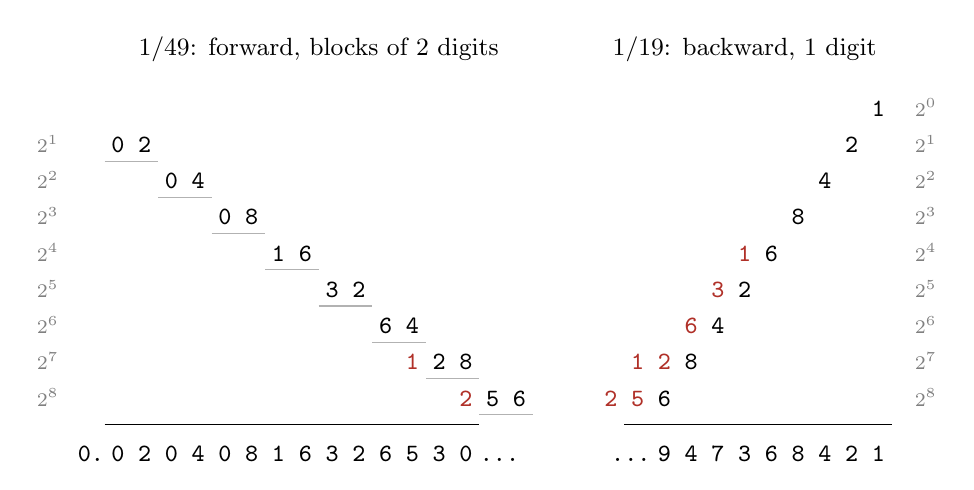
\begin{tikzpicture}[
  dig/.style={font=\ttfamily\small, inner sep=0pt, minimum width=3.2mm, anchor=base},
  ovf/.style={dig, text=ovfcol, font=\ttfamily\small\bfseries},
  lab/.style={font=\scriptsize, text=gray, anchor=base},
  ttl/.style={font=\small},
  blk/.style={gray!60, line width=0.4pt}]
\begin{scope}
\node[dig] at (0.340,-0.560) {0};
\node[dig] at (0.680,-0.560) {2};
\draw[blk] (0.170,-0.670) -- (0.850,-0.670);
\node[lab] at (-0.550,-0.560) {$2^{1}$};
\node[dig] at (1.020,-1.020) {0};
\node[dig] at (1.360,-1.020) {4};
\draw[blk] (0.850,-1.130) -- (1.530,-1.130);
\node[lab] at (-0.550,-1.020) {$2^{2}$};
\node[dig] at (1.700,-1.480) {0};
\node[dig] at (2.040,-1.480) {8};
\draw[blk] (1.530,-1.590) -- (2.210,-1.590);
\node[lab] at (-0.550,-1.480) {$2^{3}$};
\node[dig] at (2.380,-1.940) {1};
\node[dig] at (2.720,-1.940) {6};
\draw[blk] (2.210,-2.050) -- (2.890,-2.050);
\node[lab] at (-0.550,-1.940) {$2^{4}$};
\node[dig] at (3.060,-2.400) {3};
\node[dig] at (3.400,-2.400) {2};
\draw[blk] (2.890,-2.510) -- (3.570,-2.510);
\node[lab] at (-0.550,-2.400) {$2^{5}$};
\node[dig] at (3.740,-2.860) {6};
\node[dig] at (4.080,-2.860) {4};
\draw[blk] (3.570,-2.970) -- (4.250,-2.970);
\node[lab] at (-0.550,-2.860) {$2^{6}$};
\node[ovf] at (4.080,-3.320) {1};
\node[dig] at (4.420,-3.320) {2};
\node[dig] at (4.760,-3.320) {8};
\draw[blk] (4.250,-3.430) -- (4.930,-3.430);
\node[lab] at (-0.550,-3.320) {$2^{7}$};
\node[ovf] at (4.760,-3.780) {2};
\node[dig] at (5.100,-3.780) {5};
\node[dig] at (5.440,-3.780) {6};
\draw[blk] (4.930,-3.890) -- (5.610,-3.890);
\node[lab] at (-0.550,-3.780) {$2^{8}$};
\draw (0.170,-4.020) -- (4.930,-4.020);
\node[dig, anchor=base east] at (0.170,-4.490) {0.};
\node[dig] at (0.340,-4.490) {0};
\node[dig] at (0.680,-4.490) {2};
\node[dig] at (1.020,-4.490) {0};
\node[dig] at (1.360,-4.490) {4};
\node[dig] at (1.700,-4.490) {0};
\node[dig] at (2.040,-4.490) {8};
\node[dig] at (2.380,-4.490) {1};
\node[dig] at (2.720,-4.490) {6};
\node[dig] at (3.060,-4.490) {3};
\node[dig] at (3.400,-4.490) {2};
\node[dig] at (3.740,-4.490) {6};
\node[dig] at (4.080,-4.490) {5};
\node[dig] at (4.420,-4.490) {3};
\node[dig] at (4.760,-4.490) {0};
\node[dig, anchor=base west] at (4.930,-4.490) {\dots};
\node[ttl] at (2.890,0.750) {$1/49$: forward, blocks of 2 digits};
\end{scope}
\begin{scope}
\node[dig] at (10.000,-0.100) {1};
\node[lab] at (10.600,-0.100) {$2^{0}$};
\node[dig] at (9.660,-0.560) {2};
\node[lab] at (10.600,-0.560) {$2^{1}$};
\node[dig] at (9.320,-1.020) {4};
\node[lab] at (10.600,-1.020) {$2^{2}$};
\node[dig] at (8.980,-1.480) {8};
\node[lab] at (10.600,-1.480) {$2^{3}$};
\node[dig] at (8.640,-1.940) {6};
\node[ovf] at (8.300,-1.940) {1};
\node[lab] at (10.600,-1.940) {$2^{4}$};
\node[dig] at (8.300,-2.400) {2};
\node[ovf] at (7.960,-2.400) {3};
\node[lab] at (10.600,-2.400) {$2^{5}$};
\node[dig] at (7.960,-2.860) {4};
\node[ovf] at (7.620,-2.860) {6};
\node[lab] at (10.600,-2.860) {$2^{6}$};
\node[dig] at (7.620,-3.320) {8};
\node[ovf] at (7.280,-3.320) {2};
\node[ovf] at (6.940,-3.320) {1};
\node[lab] at (10.600,-3.320) {$2^{7}$};
\node[dig] at (7.280,-3.780) {6};
\node[ovf] at (6.940,-3.780) {5};
\node[ovf] at (6.600,-3.780) {2};
\node[lab] at (10.600,-3.780) {$2^{8}$};
\draw (6.770,-4.020) -- (10.170,-4.020);
\node[dig] at (10.000,-4.490) {1};
\node[dig] at (9.660,-4.490) {2};
\node[dig] at (9.320,-4.490) {4};
\node[dig] at (8.980,-4.490) {8};
\node[dig] at (8.640,-4.490) {6};
\node[dig] at (8.300,-4.490) {3};
\node[dig] at (7.960,-4.490) {7};
\node[dig] at (7.620,-4.490) {4};
\node[dig] at (7.280,-4.490) {9};
\node[dig, anchor=base east] at (7.110,-4.490) {\dots};
\node[ttl] at (8.300,0.750) {$1/19$: backward, 1 digit};
\end{scope}
\end{tikzpicture}

\caption{The two additions side by side, with the term $2^k$ on row $k$ in
both panels. In the left panel $2^k$ is written in the $k$-th two-digit block
of $1/49$. From $2^7 = 128$ on, a term no longer fits its block, and its
leading digit (red) spills into the block on its left. Grey rules mark each
term's own block. In the right panel $2^k$ is written ending $k$ places from
the right of the period of $1/19$, and every digit of a term other than its
last digit (red) is overflow into the places on its left. Adding the rows
gives the digits under the line, which agree with
$1/49 = 0.02040816326530\dots$ and with the last nine digits $947368421$ of
the period of $1/19$.}
\label{fig:additions}
\end{figure}

%======================================================================
\section{Recurrences beyond geometric series}\label{sec:recurrences}
%======================================================================

Theorems~\ref{thm:forward} and~\ref{thm:backward} sum the geometric sequences $m r^k$ and $b c^k$ by evaluating their generating functions at $t = 10^{-x}$ in $\mathbb{R}$ and at $t = 10^x$ in $\Ztena$. The Fibonacci examples $1/89$ and $1/109$ evaluate at the same two points the generating function of a recurrence of order two, where $F_k$ is the $k$-th Fibonacci number with $F_1 = F_2 = 1$. With
\begin{equation}\label{eq:G}
G(t) = \frac{t}{1 - t - t^2} = \sum_{k\ge1} F_k t^k
\end{equation}
we get, for $x = 1$,
\begin{align}
\frac{1}{89} &= \frac{G(1/10)}{10} = \sum_{k\ge1}\frac{F_k}{10^{k+1}}
  && \text{in } \mathbb{R}, \label{eq:fib}\\
-\frac{1}{109} &= \frac{G(10)}{10} = \sum_{k\ge1} F_k\, 10^{k-1}
  && \text{in } \Ztena . \label{eq:fib109}
\end{align}
The identity \eqref{eq:fib109} holds because the series converges in $\Ztena$ and satisfies $(1 - 10 - 100)\sum_{k\ge1} F_k 10^k = 10$, and because the factor $1 - 10 - 100 = -109$ is congruent to $1$ modulo $10$ and is therefore a unit in $\Ztena$ that can be divided out. The denominators are
$10^2 - 10 - 1$ and $10^2 + 10 - 1$, and the period of $1/109$ ends
$\dots 23853211$. Long~\cite{long1981} and Bicknell-Johnson~\cite{bicknell1989}
derive these and many relatives. More generally, a sequence $a_k$ with rational generating function $G(t) = \sum a_k t^k$ that converges at $t = 10^{-x}$
appears in successive $x$-digit blocks of $G(10^{-x})/10^x = \sum a_k 10^{-x(k+1)}$, with the term $a_k$ in block $k+1$ and with carries once the terms exceed $x$ digits. For $a_k = m r^k$ this is Theorem~\ref{thm:forward},
which gives the carries exactly. For $x = 2$ it gives the powers of $2$ in
$1/98$, the Fibonacci numbers in $1/9899$ and the natural numbers in
$1/9801$~\cite{munafo}.

The denominators can be read from the recurrence. Let $a_k$ be the sequence
of order $d$ given by $a_k = q_1 a_{k-1} + \dots + q_d a_{k-d}$ for $k \ge 2$
with integers $q_1, \dots, q_d$, $a_1 = 1$ and $a_k = 0$ for $k \le 0$. Then
$\sum_{k\ge1} a_k t^k = t/(1 - q_1 t - \dots - q_d t^d)$, because multiplying
the series by $1 - q_1 t - \dots - q_d t^d$ leaves only the term $a_1 t = t$.
Put
\begin{equation}\label{eq:recden}
N = 10^{dx} - q_1 10^{(d-1)x} - \dots - q_d ,
\qquad
N' = q_d 10^{dx} + \dots + q_1 10^{x} - 1 .
\end{equation}
At $t = 10^{-x}$ the generating function equals $10^{(d-1)x}/N$, and at
$t = 10^x$ it equals $-10^x/N'$. Dividing by $10^{(d-1)x}$ and by $10^x$
respectively gives
\begin{equation}\label{eq:recseries}
\frac1N = \sum_{k\ge1} \frac{a_k}{10^{x(k+d-1)}} \ \text{ in } \mathbb{R},
\qquad
-\frac1{N'} = \sum_{k\ge1} a_k\, 10^{x(k-1)} \ \text{ in } \Ztena .
\end{equation}
The real series is K\"ohler's formula for recurrences of arbitrary
order~\cite{kohler1985}, evaluated at $10^x$. To the author's knowledge the
$10$-adic series has been stated only for examples of Fibonacci and tribonacci
type, read from the right~\cite{bicknell1989}. The real series converges when
all roots of the polynomial $z^d - q_1 z^{d-1} - \dots - q_d$ are smaller than
$10^x$ in absolute value, and then $N$, the value of this polynomial at
$z = 10^x$, is positive. The $10$-adic series always converges, because its
terms are integers times $10^{x(k-1)}$, which tend to $0$. The number
$-N' = 1 - q_1 10^x - \dots - q_d 10^{dx}$ is congruent to $1$ modulo $10$, so
it is a unit in $\Ztena$ and can be divided out. For the Fibonacci numbers
$q_1 = q_2 = 1$ and $x = 1$ give $N = 89$ and $N' = 109$. For the Pell numbers
$1, 2, 5, 12, 29, 70, 169, \dots$, where $q_1 = 2$ and $q_2 = 1$, the block
length $x = 2$ gives $N = 9799$ and
$1/9799 = 0.00\,01\,02\,05\,12\,29\,71\dots$ in blocks of two digits. The block
$71$ is the term $70$ plus the carry $1$ from the next term $169$. The block
length $x = 1$ gives $N = 79$ and $N' = 119$. Hence $1/79 = 0.0126582\dots$ is
the sum $0.01 + 0.002 + 0.0005 + 0.00012 + 0.000029 + \dots$ of the Pell
numbers written one place apart, and $79$ is a denominator of
Table~\ref{tab:patterns}. The period of $1/119$ ends
$\dots 302521 = 1 + 2\cdot 10 + 5\cdot 10^2 + 12\cdot 10^3 + 29\cdot 10^4$,
which is the $10$-adic series read from the right.
These Pell examples are listed without proof in the OEIS~\cite{oeisA000129}.

The denominator $89$ also has geometric readings in both directions. Since
$100 = 1\cdot 89 + 11$, Theorem~\ref{thm:forward} gives $1/89$ as powers of $11$
in two-digit blocks, and since $89 = 10\cdot 9 - 1$, Theorem~\ref{thm:backward}
gives powers of $9$ from the right.

%======================================================================
\section{Table}
%======================================================================

Table~\ref{tab:patterns} lists, for the denominators in~\cite{mse1365506},
forward and backward patterns written as \emph{first block} $\times$
\emph{multiplier}$^k$, with the Fibonacci numbers listed by name. For each $n$
the block lengths $x \le 3$ were chosen by hand to give a small multiplier. The
forward and backward entries in a row may use different $x$, and by
Remark~\ref{rem:dual} a forward multiplier for $x$ is the backward multiplier
for $L - x$. The rows for $7$, $19$, $49$, $83$ and $199$ come from
Proposition~\ref{prop:T} with $T = 50$, $20$, $50$, $250$ and $200$. All
entries were checked by exact computation (Appendix~\ref{app:code}).

\begin{table}[ht]
\centering
\begin{tabular}{rrll}
\toprule
$n$ & $L$ & forward (left to right) & backward (right to left) \\
\midrule
7   & 6   & $x=2$: $14\times 2^k$   & $x=1$: $7\times 5^k$ \\
19  & 18  & $x=2$: $05\times 5^k$   & $x=1$: $1\times 2^k$ \\
47  & 46  & $x=2$: $02\times 6^k$   & $x=2$: $17\times 8^k$ \\
49  & 42  & $x=2$: $02\times 2^k$   & $x=1$: $1\times 5^k$ \\
71  & 35  & $x=3$: $014\times 6^k$  & $x=3$: $169\times 12^k$ \\
79  & 13  & $x=2$: $01\times 21^k$  & $x=1$: $1\times 8^k$ \\
83  & 41  & $x=3$: $012\times 4^k$  & $x=1$: $3\times 25^k$ \\
89  & 44  & $x=1$: Fibonacci        & $x=1$: $1\times 9^k$ \\
97  & 96  & $x=2$: $01\times 3^k$   & $x=1$: $7\times 68^k$ \\
109 & 108 & $x=3$: $009\times 19^k$ & $x=1$: Fibonacci or $1\times 11^k$ \\
199 & 99  & $x=3$: $005\times 5^k$  & $x=2$: $01\times 2^k$ \\
\bottomrule
\end{tabular}

\vspace{8pt}
\caption{Forward and backward patterns for the denominators of~\cite{mse1365506}.}
\label{tab:patterns}
\end{table}

%======================================================================
\section{Classroom use}\label{sec:classroom}
%======================================================================

The results above join four topics that students meet separately. Long division produces the digits. The geometric series explains the forward patterns. The inverse of $10^x$ modulo $n$, which the extended Euclidean algorithm computes, gives the backward multiplier $c$. The backward series is a first example of a $10$-adic number, namely $-1/n$ with its expansion $\dots PPP$. Theorem~\ref{thm:forward} also lets a student predict the carries. The first block that differs from its term is the one with the least $k$ for which $\lfloor r^{k+1}/n \rfloor \ge 1$, and for $r \ge 2$ this is the block with $k = \lceil \log n/\log r \rceil - 1$. The following exercises use only the results above and elementary arithmetic.

\begin{enumerate}
\item Show that $1/29$ triples from the right, so that its period ends in
  $1, 3, 9, 27, \dots$ written one place further left each time. Find every
  denominator whose period triples from the right in two-digit blocks.
\item Use Theorem~\ref{thm:forward} with $1000 = 2\cdot 499 + 2$ to predict how many powers of $2$ appear unchanged in the three-digit blocks of $1/499$, and which block shows the first carry.
\item Apply Proposition~\ref{prop:T} with $T = 40$ to $n = 39$. Show that
  $1/39$ follows the powers of $25$ forward in three-digit blocks and the
  powers of $4$ backward in one-digit blocks, and check both against
  $1/39 = 0.\rep{025641}$.
\item The forward multiplier of $1/7$ for $x = 1$ is $3$. Use Remark~\ref{rem:dual} to find the block length $x$ with $1 \le x < 6$ in which $1/7$ triples from the right, and confirm it with the period $142857$.
\end{enumerate}

The answers are as follows. In the first exercise $3\cdot 10 - 1 = 29$, so $3$ is the inverse of $10$ modulo $29$, and Theorem~\ref{thm:backward} with $x = 1$, $c = 3$ and $b = 1$ shows that $1/29$ triples from the right. For blocks of $x$ digits the multiplier is $c = 3$ exactly when $n > 3$ and $n \mid 3\cdot 10^x - 1$. For $x = 2$ this number is $299 = 13\cdot 23$, so the denominators are $13$, $23$ and $299$. In the second, $m = r = 2$, so the terms are $2^{k+1}$. The inequality $2^{k+1} < 499$ holds for $k \le 7$, so the eight terms $002, 004, \dots, 256$ appear unchanged, and the ninth block is $512 + \lfloor 512/499 \rfloor = 513$. In the third, $T - 1 = 39$ gives $b = 1$. Next, $T = 10\cdot 4$ gives $x = 1$ and $c = 4 < 39$, and $25\cdot 40 = 1000$ gives $x' = 3$ and $r = 25 < 39$, so the hypotheses of Proposition~\ref{prop:T} hold with $m = rb = 25$. The first block is $025$ and the second is $625 + \lfloor 625/39 \rfloor = 641$. From the right, $c = 4$ gives the terms $1, 4, 16, 64, \dots$, each one place further left, and their sum modulo $10^6$ is $025641$. In the fourth, $L = 6$, so $1/7$ triples from the right in blocks of length $6 - 1 = 5$. Here $c = 3$ and $b = (3\cdot 10^5 - 1)/7 = 42857$, which are the last five digits of $142857$.

%======================================================================
\section{Further directions}
%======================================================================

For $r \ge 2$ the number $\lceil \log n/\log r \rceil - 1$ of terms printed unchanged depends on the block length $x$ through $r$. Its largest value over the block lengths $x$ with $10^x > n$ and $r \ge 2$ is finite and could rank all denominators below a bound by the length of the unchanged run of terms in their expansions. The theorems and their proofs hold
with $10$ replaced by any base $B \ge 2$ and $n$ coprime to $B$, and MathPages
works out examples in base $6$~\cite{mathpages859}.

\section*{Acknowledgements}
The author thanks David~K.\ for his answers~\cite{mse1365506,mse1372077}.

\section*{Use of artificial intelligence}
The question and its examples are the author's own work from
2015~\cite{mse1365506}. In 2026 the author wrote this article from them with
NeuroPaja, a setup in which the AI agents Anthropic Claude, OpenAI Codex and
Google Antigravity helped with the literature, the text, the proofs and the
checks. Every number and stated result is checked by exact computation on small
cases, and the author is responsible for the content.

\appendix
\section{Computational checks}\label{app:code}

The repository \url{https://github.com/markomanninen/multiplier-patterns} accompanying this article contains \texttt{verify.py}, which checks
every number in the text with exact integer arithmetic, and
\texttt{derivations.mac}, a Maxima session that derives the closed forms. A
representative excerpt:

\begin{lstlisting}
row(n, x) := block([X : 10^x, m, r, c, b],
  m : floor(X/n), r : X - m*n,
  c : inv_mod(X, n), b : (X*c - 1)/n,
  [n, zn_order(10, n), x, m, r, b, c, is(equal(mod(r*c, n), 1))])$
row(19, 1);   /* [19, 18, 1, 0, 10, 1, 2, true], m = 0 */
row(19, 2);   /* [19, 18, 2, 5, 5, 21, 4, true] */
ifactors(2*10^6 - 1);   /* [[17,1],[71,1],[1657,1]] */
\end{lstlisting}

\bibliographystyle{amsplain-full}
\bibliography{refs}

\end{document}
